\documentclass[a4paper,12pt]{article}
\usepackage[utf8]{inputenc}
\usepackage{graphicx}
\usepackage{amsmath}
\usepackage{hyperref}
\usepackage{geometry}
\usepackage{float}
\geometry{margin=1in}

\begin{document}

\title{Handwritten Signature Detection and Localization in Documents}
\author{Federico Iannini, Andrea Puddu, Riccardo Pitzanti \\
\small Foundations of Data Science – Sapienza University of Rome}
\date{December 2024}
\maketitle

\begin{abstract}
% !TODO revise
Localizing handwritten signatures in scanned documents is useful for automating workflows in industries such as legal, banking, and archival systems. This report explores three distinct approaches to address this task: a naive grid-based method, a selective search-based approach leveraging image features, and a state-of-the-art Faster R-CNN model. Each method is evaluated for its ability to propose and classify regions of interest, with selective search dynamically adapting to document characteristics and Faster R-CNN providing the highest accuracy via end-to-end training. The pipeline integrates preprocessing techniques, including edge detection and image filters, to enhance signature localization accuracy. Results demonstrate the trade-offs between simplicity, computational efficiency, and performance across the approaches. Future work aims to further optimize region proposal strategies, explore advanced architectures and expand towards broader use cases.
\end{abstract}

\section{Introduction}
%!TODO improve
This project focuses on automating the detection and localization of handwritten signatures in scanned documents. By identifying and bounding signatures, the pipeline reduces manual labor and improves workflow efficiency in industries like legal and banking. The approach integrates machine learning, edge detection techniques, and region-based localization to handle diverse document formats and scenarios. 

\section{Related Work}
%!TODO reference more sources.
Handwritten signature detection has been a key area of research. Wu et al.~\cite{wu2021} introduced object detection models for handwriting localization, while Cüceloğlu and Oğul~\cite{cuceloglu2018} developed a specific method for detecting signatures in scanned documents. Selective search, introduced by Uijlings et al.~\cite{victor2013}, is used here for bounding box initialization, enabling efficient region proposal generation.

\section{Dataset}
%!TODO revise
The dataset, SignverOD, consists of 2765 scanned document images with 7103 bounding boxes annotated across four categories: handwritten signatures, initials, redactions, and dates. For this project, the focus is solely on the "signature" category. These documents are sourced from diverse repositories, including Tobacco800, NIST.gov Special Database, a bank checks dataset, and GSA lease documents, for a broad representation of document types. All documents in the dataset vary in size, with bounding box annotations provided in normalized coordinates relative to document dimensions. The dataset is split into 1991 training images, 221 for validation, and 553 for testing, with 4451 bounding boxes specifically annotated as signatures. To further support the model, non-signature crops are generated by masking annotated signature regions and extracting random patches, creating a balanced dataset necessary for training a binary classifier.

\section{Pipeline Implementation}
%!TODO revise the whole section
The pipeline is designed to pre-process data, train models, and localize signatures effectively. Key steps include:

\subsection{Data Pre-processing}
Data pre-processing involves:
\begin{itemize}
    \item \textbf{Download of the Dataset}: The dataset is downloaded from Kaggle~\cite{dataset} and then fixed (see:~\cite{dataset_fix}). Train and test files are merged in order to ensure a custom split of data.
    \item \textbf{Cropping Signatures}: Images are cropped to bounding boxes around their respective annotated signatures.
    \item \textbf{Resizing}: Cropped signatures are resized to a uniform dimension to standardize input for the CNN. This uniform dimension is obtained by computing the mean height and width of all the documents (734x177 pixels).
    \item \textbf{Non-Signature Generation}: Using masked images, non-signature regions are extracted, avoiding overlap with annotated signatures.
    \item \textbf{Image pre-processing}: If specified, edge detection techniques such as Canny, Sobel, and Laplacian are employed. It is possible to choose also a Gaussian filter, a binary mask threshold or no pre-processing at all.
\end{itemize}

\subsection{Model Training}

The goal of the model is to classify sections of a document as either containing a handwritten signature or not. The training data consist of cropped and preprocessed sections of documents, where each crop is labeled as either a signature or a non-signature.
Given that the input data are images, we used a CNN structure.
The architecture used in this project is shown in Figure~\ref{fig:cnn_architecture}. It is a relatively simple model that consists in a few layers: \begin{itemize} \item \textbf{Convolutional Layer}: Extracts spatial features from the input image using filters, followed by a Leaky ReLU activation function. \item \textbf{Batch Normalization}: Normalizes the activations to accelerate training and reduce sensitivity to initialization. \item \textbf{Max-Pooling Layer}: Reduces the spatial dimensions of the feature maps while retaining the most salient information. \item \textbf{Dense Layers}: Fully connected layer maps the extracted features to a binary classification output for which the sigmoid activation function is used. \end{itemize}

We experimented with deeper architectures (e.g., more convolutional layers, dropout for regularization), but observed that even this minimal configuration achieved excellent performance, with an accuracy of approximately 97\% and a low binary cross-entropy loss. Given this performance and to optimize resources usage, we selected this simple architecture to reduce training time and computational costs while maintaining high accuracy.

\begin{figure}[H]
    \centering
    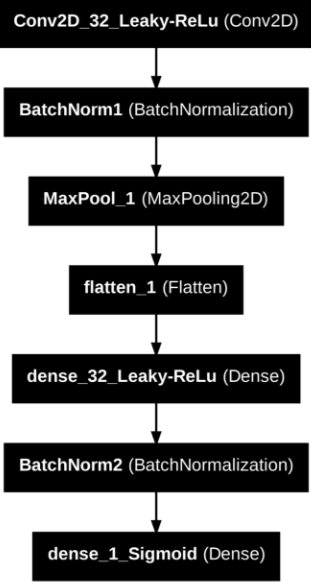
\includegraphics[scale=0.7]{signmodel.png}
    \caption{CNN Architecture used for Signature Detection.}
    \label{fig:cnn_architecture}
\end{figure}

This lightweight network proved to be effective and efficient for the task at hand, providing a robust foundation for classifying document sections for the signature detection pipeline.

\subsection{Region Proposal and Classification}
During testing, bounding box proposals are generated by leveraging one of two different approaches (see Section 5). These regions are classified as containing signatures or not using the trained CNN. Detected regions with a confidence score above a threshold ($\ge$ 90\%) are retained.

\subsection{Post-Processing}
Bounding boxes are merged if they overlap significantly (IoU $\ge$ 40\%). They are then rescaled and saved with their confidence scores.


\section{Methods}
%!TODO revise
At first, we decided to implement a naive method from scratch, that relies on a fixed grid approach to divide documents into uniform regions. These regions are then passed to the binary classifier CNN, trained to differentiate between signature and non-signature areas. The naive approach does not dynamically adapt region proposals to document features. The lack of a mechanism to prioritize regions likely to contain signatures results in an increased computational cost, as the model processes many irrelevant regions.

The selective search-based method improves upon the naive approach by introducing a dynamic region proposal mechanism. Instead of dividing the document into a fixed grid, selective search identifies potential regions of interest dynamically. The approach begins by extracting ink-detected regions from the document to locate high-gradient areas, which are indicative of potential signature placements. A set of bounding boxes is then initialized at random coordinates within these ink-detected parts of the document. The size and aspect ratio of these bounding boxes are scaled relative to a precomputed "base dimension", derived from the average dimensions of annotated bounding boxes in the training dataset. To introduce variability, oscillating factors are applied to the width and height of the base dimension, resulting in varied bounding boxes. Each bounding box is then classified by the CNN, which determines whether it contains a signature. Only bounding boxes with classification confidence scores exceeding a specified threshold are retained. This approach significantly reduces the number of irrelevant regions passed to the classifier, prioritizing areas more likely to contain signatures. Finally, overlapping bounding boxes are merged in a post-processing step using Intersection over Union (IoU) metrics. This ensures non-redundant predictions. Compared to the naive approach, this method dynamically adapts to document features and leverages edge detection to propose meaningful regions for classification, improving both accuracy and computational efficiency.

The third approach regards a Faster R-CNN model, a state of the art object detection framework widely used for region-based tasks. Unlike the pipeline described above, Faster R-CNN combines region proposal and classification into a single, end-to-end trainable model. The model consists of a Region Proposal Network (RPN) that generates potential bounding boxes directly from image features. These proposals are refined and classified in subsequent network layers. The Faster R-CNN used in this project is implemented in PyTorch and fine-tuned on the SignverOD dataset. Its architecture allows it to learn spatial hierarchies and detect signatures of varying sizes and orientations. While the Faster R-CNN achieves superior performance in terms of accuracy and IoU, it requires more computational resources and longer inference times compared to the selective search-based method.


\section{Performance Evaluation}
Performance is measured for both methods (naive and selective search) using precision, recall, F1 score, and IoU metrics. A bounding box is considered a true positive if its IoU with the ground truth is above 0.4. The iterative localization process ranks regions by confidence, removing overlapping predictions. These performances are then compared with the results obtained by the Faster-RCNN.

\section{Results}
%!TODO Insert graph comparison, or (better) table.



\section{Conclusion(?) and Future Work}
% !TODO expand
Future work includes refining region proposal methods, incorporating advanced models like YOLO, and extending functionality to include forgery detection.

\section{Roles}
\begin{itemize}
    \item \textbf{Data pre-processing, first region proposal algorithm implementation}: Federico, Riccardo
    \item \textbf{Selective search and CNN model}: Federico
    \item \textbf{Performance evaluation and data visualization}: Riccardo
    \item \textbf{Faster R-CNN}: Andrea
\end{itemize}

\begin{thebibliography}{9}
\bibitem{wu2021} Wu, Yuli, Yucheng Hu, and Suting Miao. "Object Detection Based Handwriting Localization." \textit{arXiv preprint} (2021). Available online: \url{https://arxiv.org/pdf/2106.14989}.
\bibitem{cuceloglu2018} Cüceloğlu, İlkhan, and Hasan Oğul. "Detecting handwritten signatures in scanned documents." \textit{ResearchGate} (2018). Available online: \url{https://www.researchgate.net/publication/326271482}.
\bibitem{victor2013} Uijlings, J.R.R., et al. "Selective Search for Object Recognition." \textit{International Journal of Computer Vision} (2013). Available online: \url{https://ivi.fnwi.uva.nl/isis/publications/2013/UijlingsIJCV2013/UijlingsIJCV2013.pdf}.
\bibitem{dataset} "SignverOD Dataset." Kaggle. Available online: \url{https://www.kaggle.com/datasets/victordibia/signverod}.
\bibitem{dataset_fix} "Fixing the SignverOD Dataset." Kaggle. Available online: \url{https://www.kaggle.com/code/alexhorduz/fixing-signverod-dataset}.
\end{thebibliography}


\end{document}
